\documentclass[12pt]{article}

% ============================================================
% Shared preamble — paper and talks
% See .claude/rules/working-paper-format.md for standards.
% ============================================================

% ====== Page Layout and Basic Formatting ======
\usepackage[left=1.0in,right=1.0in,top=1.0in,bottom=1.0in]{geometry}
\usepackage{setspace}
\doublespacing
\usepackage{fancyhdr}
\pagestyle{fancy}
\fancyhf{}
\fancyfoot[C]{\thepage}
\renewcommand{\headrulewidth}{0pt}

% ====== Typography and Fonts ======
\usepackage{lmodern}
\usepackage{microtype}
\usepackage[normalem]{ulem}
\usepackage[T1]{fontenc}

% ====== Section Styling ======
\usepackage{titlesec}
\usepackage[title]{appendix}
\usepackage{titling}
\pretitle{\begin{center}\large\bfseries}
\posttitle{\end{center}}
\preauthor{\begin{center}\normalsize}
\postauthor{\end{center}}
\predate{\begin{center}\normalsize}
\postdate{\end{center}}

% ====== Math Packages ======
\usepackage{amssymb, amsmath, amsfonts, mathtools}
\usepackage{dsfont}
\usepackage{amsthm}
\newtheorem{theorem}{Theorem}
\newtheorem{proposition}{Proposition}
\newtheorem{corollary}{Corollary}
\newtheorem{lemma}{Lemma}
\newtheorem{definition}{Definition}
\newtheorem{hyp}{Hypothesis}
\DeclareMathOperator*{\argmax}{arg\,max}
\DeclareMathOperator*{\argmin}{arg\,min}
\newcommand{\norm}[1]{\left\lVert #1 \right\rVert}
\newcommand{\1}[1]{\mathds{1}\left[#1\right]}

% ====== Table Packages ======
\usepackage{array, booktabs, makecell, cellspace}
\usepackage{siunitx}
\usepackage[flushleft]{threeparttable}
\usepackage{rotating, tabularx}
\usepackage{tabularray}
\UseTblrLibrary{booktabs, siunitx}

% ====== Figure and Caption Packages ======
\usepackage{graphicx, subcaption}
\usepackage{pdflscape, tikz}
\usepackage{caption}
\captionsetup{font=small, labelfont=bf, justification=justified}
\captionsetup[figure]{labelfont=bf}
\usepackage{float}

% ====== List Formatting ======
\usepackage{enumitem}

% ====== Bibliography and Citation (biblatex-apa, APA 7) ======
\usepackage{xurl}
\usepackage{xcolor}
\definecolor{citationcolor}{RGB}{0, 127, 255}
\usepackage{csquotes}

\usepackage[backend=biber,
            style=apa,
            natbib=true,
            uniquename=false,
            uniquelist=true,
            sortcites=true,
            maxcitenames=2,
            mincitenames=1,
            maxbibnames=99,
            minbibnames=99,
            giveninits=false
            ]{biblatex}
% Keep English-APA mapping for the bibliography (cited works are in English).
% Document body language is set to Spanish via babel below.
\DeclareLanguageMapping{english}{english-apa}

\DeclareCiteCommand{\cite}
  {\usebibmacro{prenote}}
  {\usebibmacro{citeindex}%
   \printtext[bibhyperref]{\color{citationcolor}\usebibmacro{cite}}}
  {\multicitedelim}
  {\usebibmacro{postnote}}
\DeclareCiteCommand{\parencite}[\mkbibparens]
  {\usebibmacro{prenote}}
  {\usebibmacro{citeindex}%
   \printtext[bibhyperref]{\color{citationcolor}\usebibmacro{cite}}}
  {\multicitedelim}
  {\usebibmacro{postnote}}

% ====== Custom Column Types ======
\newcolumntype{L}[1]{>{\raggedright\let\newline\\\arraybackslash\hspace{0pt}}m{#1}}
\newcolumntype{C}[1]{>{\centering\let\newline\\\arraybackslash\hspace{0pt}}m{#1}}
\newcolumntype{R}[1]{>{\raggedleft\let\newline\\\arraybackslash\hspace{0pt}}m{#1}}

% ====== Footnote Settings ======
\interfootnotelinepenalty=10000
\setlength{\footnotesep}{0.5cm}

% ====== URL Bleeding Fixes ======
\setcounter{biburllcpenalty}{7000}
\setcounter{biburlucpenalty}{8000}
\setcounter{biburlnumpenalty}{9000}

% ====== Babel (Spanish document body) ======
\usepackage[spanish,es-tabla,es-noindentfirst]{babel}

% ====== Hyperref (second-to-last) ======
\usepackage[hidelinks, breaklinks, colorlinks=true,
            linkcolor=citationcolor, citecolor=citationcolor,
            urlcolor=citationcolor]{hyperref}

% ====== Cleveref (after hyperref) ======
\usepackage[nameinlink,spanish]{cleveref}
% Forzar nombres en espanol (cleveref a veces deja ingles aun con la opcion).
\crefname{section}{secci\'{o}n}{secciones}
\Crefname{section}{Secci\'{o}n}{Secciones}
\crefname{subsection}{subsecci\'{o}n}{subsecciones}
\Crefname{subsection}{Subsecci\'{o}n}{Subsecciones}
\crefname{subsubsection}{subsecci\'{o}n}{subsecciones}
\Crefname{subsubsection}{Subsecci\'{o}n}{Subsecciones}
\crefname{table}{tabla}{tablas}
\Crefname{table}{Tabla}{Tablas}
\crefname{figure}{figura}{figuras}
\Crefname{figure}{Figura}{Figuras}
\crefname{equation}{ecuaci\'{o}n}{ecuaciones}
\Crefname{equation}{Ecuaci\'{o}n}{Ecuaciones}
\crefname{appendix}{ap\'{e}ndice}{ap\'{e}ndices}
\Crefname{appendix}{Ap\'{e}ndice}{Ap\'{e}ndices}

\addbibresource{../Bibliography_base.bib}

\title{The Labor Market Impact of Generative AI:\\ Causal Evidence from Latin America\thanks{Pontificia Universidad Cat\'{o}lica del Per\'{u} (PUCP), Programa Doctoral en Econom\'{i}a. Contact: \texttt{etorres@pucp.edu.pe}. I thank my advisors and the PUCP labor reading group for comments. This paper extends joint work with Oliver Azuara and Laura Ripani at the Inter-American Development Bank \citep{Azuara2024_idb_ai}. All errors are my own.}}

\author{Eric Torres}

\date{\today}

\begin{document}

\maketitle
\thispagestyle{empty}

\begin{abstract}
\noindent \singlespacing
The launch of ChatGPT in November 2022 delivered a common, exogenous shock to labor markets worldwide, yet the only careful causal estimates come from OECD economies where informality is low and digital adoption is high. This paper provides the first causal estimates of how exposure to large language models (LLMs) affected employment, hours, and wages in Latin America. Using harmonized labor force surveys from seven countries (2021Q1--2025Q4), occupational exposure scores from \citet{Eloundou2023_gpt_exposure}, and the continuous-treatment difference-in-differences estimator of \citet{CallawayCGBS2024_continuous}, I estimate the Average Causal Response on the Treated along the dose dimension. Baseline (2021) formality is pre-registered as the central heterogeneity margin. I contrast the results with the near-null Danish estimates of \citet{HumlumVestergaard2025_llm} and test four pre-committed narratives in which informality either amplifies, buffers, or reallocates the shock.

\vspace{1em}
\noindent \textbf{JEL Codes:} J23, J31, O33, O54, D63, L86

\vspace{0.5em}
\noindent \textbf{Keywords:} generative AI, large language models, labor demand, wage inequality, informality, Latin America, difference-in-differences
\end{abstract}

\newpage
\setcounter{page}{1}

\section{Introduction}
\label{sec:introduction}

Generative artificial intelligence is widely expected to be the defining labor-market shock of the 2020s. The launch of ChatGPT on 30 November 2022 gave the world's first general-purpose large language model (LLM) to hundreds of millions of users within months, and occupational exposure measures suggest that roughly half of US jobs have at least one task that LLMs can perform twice as fast as a human \citep{Eloundou2023_gpt_exposure}. Against these projections, the first set of careful causal estimates is striking. \citet{HumlumVestergaard2025_llm} use Danish administrative data linked to a 100{,}000-worker adoption survey and rule out wage and hours effects larger than two percent, two years after launch. Two-percent effects are economically small. They are also geographically narrow: essentially every credible causal estimate of how LLMs have reshaped aggregate labor markets comes from the United States, Denmark, or online freelance platforms in which workers in advanced economies dominate.

This leaves the first-order question - whether the most widely hyped general-purpose technology of the decade has actually moved labor-market outcomes - essentially unresolved for the developing world. Latin America is the natural place to ask. The region's aggregate informality rate sits near 55 percent, with country-specific rates between 25 percent in Uruguay and more than 70 percent in parts of the Andean region. Formal and informal workers occupy segmented markets with different wage-setting institutions, different degrees of exposure to digital technology, and different buffers against productivity shocks. Exposure to LLMs in Latin America is also structurally different: \citet{Azuara2024_idb_ai} show that predicted exposure tilts sharply toward formal, female, urban, and tertiary-educated workers in Chile, Mexico, and Peru, and \citet{Ciaschi2025_distributive_ai} and \citet{EganadelSol2025_ai_lac} extend this exposure-only picture to the broader region. What no existing paper provides is a causal estimate of whether this exposure has translated into actual labor-market responses.

This paper fills that gap. I assemble a harmonized panel of seven Latin American labor force surveys (Peru, Uruguay, Mexico, Chile, Colombia, Costa Rica, and Ecuador) covering 2021Q1 through 2025Q4, map Eloundou et al.'s occupational exposure scores from SOC-2010 to ISCO-08 via the BLS crosswalk (match rate 98.2 percent at the 4-digit level), and estimate the Average Causal Response on the Treated (ACRT) along the continuous exposure dimension using the difference-in-differences estimator of \citet{CallawayCGBS2024_continuous}. The post-COVID time window is a deliberate design choice: including pre-2020 periods would pool labor markets in two structurally different equilibria, violating the comparability requirement for the DiD control group. ChatGPT's launch delivers a single adoption date common to all occupations; identification comes from within-(occupation, country) variation in how exposure interacts with the post-launch indicator. Baseline (2021) formality status is pre-registered as the paper's central heterogeneity margin, on the argument that contemporaneous formality is itself an outcome of LLM exposure and therefore a bad control.

% RESULTS TBD — four narratives pre-registered, one realized
The results fall into one of four pre-committed narratives. I state the narratives now and defer the quantitative headline numbers to \cref{sec:results}, where they appear with exposure-normalized effect sizes, confidence intervals, and Honest-DiD bounds. \emph{Narrative A} (informality amplifies): aggregate LAC effects exceed two percent and are driven by the informal channel, with $\tau_I < \tau_F < 0$. \emph{Narrative B} (LAC-Denmark null replication): aggregate effects are indistinguishable from zero in both channels. \emph{Narrative C} (null in formal, large in informal): $\tau_F \approx 0$ and $\tau_I$ is meaningfully negative, identifying a channel that Danish and US designs cannot detect because their informal sectors are negligible. \emph{Narrative D} (stratified gains): positive wage effects concentrate in tertiary-educated urban formal workers, bypassing the informal majority.

% Placeholder finding paragraphs to be activated once results arrive.
% [Narrative A finalization paragraph]: Consistent with Narrative [X]. On the full sample, a one-standard-deviation increase in Eloundou ζ exposure is associated with a [X] pp change in employment and a [X] percent change in log hourly wages post-2023. The informal channel accounts for [X] percent of the aggregate effect.

The paper's cleanest contribution is its contrast with \citet{HumlumVestergaard2025_llm}. Denmark's combination of low informality, high digital readiness, strong worker bargaining, and generous social insurance is precisely the structural configuration most likely to mute a labor-market response: buffers absorb the shock before it registers in administrative earnings data. Latin America's configuration is the opposite - high informality, fragmented wage-setting, weaker social insurance, and lower but non-trivial adoption. If the Danish null is universal, it should survive in this very different setting; if it reflects Danish institutions rather than LLM capabilities, the LAC estimates should diverge in a predictable direction. The seven-country panel sharpens this comparison by delivering within-region variation in informality (25 to 70 percent), digital penetration, and ChatGPT adoption intensity.

The mechanism is organized around the task-based framework of \citet{AcemogluRestrepo2018_race} and \citet{AcemogluAutor2011_tasks}. LLMs act simultaneously through a displacement channel (substituting for non-routine cognitive tasks) and a reinstatement channel (complementing human judgment in tasks that require contextual reasoning). The net effect on employment and wages is empirical, not theoretical, and its decomposition across formality strata is exactly what the pre-registered specification targets. LLMs also break the classical routine-biased technical change pattern of \citet{AutorLM2003_skill_content}: the tasks most affected (writing, synthesis, analysis) are non-routine cognitive tasks historically considered protected from automation.

The paper makes five contributions. First, it provides the first causal estimates of LLM exposure on labor-market outcomes for Latin America, filling the gap between the descriptive exposure literature \citep{Azuara2024_idb_ai, Ciaschi2025_distributive_ai, EganadelSol2025_ai_lac, WorldBank2024_genai_lac} and the OECD-focused causal literature \citep{HumlumVestergaard2025_llm, Hartley2024_labor_effects, Chen2025_llm_unemployment}. Second, it applies \citet{CallawayCGBS2024_continuous} continuous-treatment DiD to LLM exposure; the prior causal literature has relied on binary cutoffs, discarding most of the dose variation. Third, it elevates baseline formality from a subgroup check to the co-primary identification margin, with an imputation protocol that avoids using a post-treatment outcome as a conditioning variable. Fourth, it builds a reproducible seven-country harmonized crosswalk and panel (2021--2025) that future LAC researchers can extend. Fifth, the paper pre-commits to four narratives before the analysis is run, so that the narrative emphasized in the final draft is determined by which empirical pattern obtains rather than by post-hoc specification search.

The rest of the paper proceeds as follows. \Cref{sec:literature} places the contribution in relation to the AI exposure literature, the post-ChatGPT causal evidence, the task-based theoretical framework, and the LAC-specific context. \Cref{sec:method} presents the identification strategy, the continuous-DiD estimating equation, the four pre-registered narratives, and the robustness layer. \Cref{sec:data} describes the seven-country harmonized panel. \Cref{sec:results} reports the main estimates and the baseline-formality decomposition. \Cref{sec:robustness} presents the robustness evidence, and \Cref{sec:conclusion} discusses external validity and policy implications.

\section{Related Literature}
\label{sec:literature}

This paper sits at the intersection of four literatures: the measurement of AI exposure at the occupational level, the post-ChatGPT causal evidence on labor-market outcomes, the task-based theoretical framework for automation and inequality, and the Latin American literature on technology and informal labor markets. I organize the discussion thematically rather than chronologically.

\subsection{Measuring AI exposure}
\label{subsec:lit_exposure}

The canonical exposure measure in the LLM era is \citet{Eloundou2023_gpt_exposure}. Using GPT-4 and a human rubric, the authors rate each O*NET task on whether an LLM (possibly augmented with LLM-powered software) could reduce the time required to perform it by at least 50 percent. Three aggregate occupational scores result: $\alpha$ (direct exposure), $\beta$ (exposure with LLM-powered complementary software), and $\zeta = \alpha + \beta$ (the upper bound). I use $\zeta$ as the primary treatment, with $\alpha$, $\beta$, and alternative measures in robustness. Two alternatives precede Eloundou et al. \citet{Webb2020_ai_exposure} maps AI patents to O*NET tasks, producing an exposure measure that pre-dates generative AI and therefore isolates the pre-LLM automation component. \citet{Felten2023_ai_exposure} construct the AI Occupational Exposure index (AIOE) from expert task-capability assessments in the Electronic Frontier Foundation AI Progress Measurement dataset. These three measures converge on the coarse ranking of occupations (cognitive, language-intensive, clerical/professional work ranks highest) but differ at finer resolutions.

A concern with any predicted exposure measure is whether it reflects actual LLM use. \citet{Handa2025_economic_tasks} address this by analyzing millions of Claude conversations from Anthropic and mapping them to O*NET tasks. The realized-usage ranking correlates strongly with the Eloundou predicted-exposure ranking, which provides empirical content to the ``score-as-dose'' interpretation that I rely on throughout. For Latin America, \citet{Azuara2024_idb_ai} extend the Eloundou measure to Chile, Mexico, and Peru using the BLS SOC-to-ISCO crosswalk, which I build on.

\subsection{Causal effects of LLMs on labor markets}
\label{subsec:lit_causal}

The causal literature is young and growing fast. Firm- and task-level evidence, which comes closest to identifying a clean productivity effect, is generally positive. \citet{Brynjolfsson2023_genai} run a randomized rollout of an LLM-based assistant in a US customer-service call center and document a 14 percent productivity gain concentrated among less-experienced workers. \citet{CuiDemirerJaffe2025_copilot} report 26 percent faster task completion for software developers across three RCTs with nearly 5{,}000 participants. These estimates bound the complementarity channel from above: in a setting where adoption is exogenously delivered, the technology works as advertised.

Aggregate labor-market evidence is more mixed. \citet{Hartley2024_labor_effects} use the US Current Population Survey and a DiD design around the ChatGPT launch to document measurable hours and wage responses in high-exposure occupations. \citet{Chen2025_llm_unemployment} apply a synthetic DiD to US data and find roughly \$89 per week higher earnings in high-exposure occupations, with no detectable effect on unemployment. \citet{Hui2024_online_labor} examine online freelance platforms and show sharp declines (20 to 50 percent) in demand for writing and translation services post-launch, with accompanying earnings drops of 2 to 5 percent. \citet{Liu2025_generate_future} reach similar conclusions in a related online-labor sample. \citet{LiuWangYu2025_labor_demand} use 285 million US job postings and estimate that high-AI-exposure occupations saw a 12 percent decline in posted positions in the first post-launch year, rising to 18 percent by year three.

Against these positive-displacement or positive-earnings estimates, \citet{HumlumVestergaard2025_llm} deliver a striking null. Using Danish administrative data linked to an adoption survey of 100{,}000 workers across eleven exposed occupations, they rule out earnings or hours effects larger than two percent two years post-launch, despite documenting widespread adoption. Their companion paper \citep{HumlumVestergaard2025_pnas} shows that this adoption is itself unequal, skewing male, young, and educated. The tension between positive micro-productivity gains (Brynjolfsson, Cui) and near-null aggregate effects (Humlum-Vestergaard) is the central unresolved question in this literature.

I position this paper as the reference-class challenge to \citet{HumlumVestergaard2025_llm}. Their null may reflect a universal feature of LLM shocks at two-year horizons, or it may reflect specifically Danish labor-market buffers. Latin America offers the opposite structural configuration: high informality, weaker bargaining institutions, and lower but non-trivial adoption. If the null survives in this very different setting, Denmark was not the exception; if it does not, informality is the margin that matters. The paper also serves as external validity for \citet{Hartley2024_labor_effects} and \citet{Chen2025_llm_unemployment}: the harmonized seven-country panel can either confirm their positive estimates in a developing-region setting or document that their magnitudes do not replicate outside the United States.

\subsection{Tasks, automation, and inequality}
\label{subsec:lit_theory}

The theoretical framework follows \citet{AcemogluAutor2011_tasks} and \citet{AcemogluRestrepo2018_race}: technology affects labor demand through two opposing channels. The \emph{displacement effect} substitutes capital (or algorithms) for labor in tasks that the technology can now perform, reducing labor demand in exposed occupations. The \emph{reinstatement effect} creates new tasks or raises the productivity of human labor in tasks complementary to the technology, raising demand in exposed occupations. The net effect on employment and wages is empirical and depends on the relative strength of the two channels. \citet{AcemogluRestrepo2022_tasks_inequality} quantify this framework for US data from 1980--2016 and attribute 50 to 70 percent of the observed rise in wage inequality to task displacement in automating industries, a result this paper's distributional analysis (Paper 2) adapts to the LLM shock.

\citet{AutorLM2003_skill_content} provide the classical routine-biased technical change (RBTC) framework: computers and industrial robots automated \emph{routine} cognitive and manual tasks, compressing wages in the middle of the distribution. LLMs break this pattern. The tasks LLMs most affect - writing, synthesis, analysis, code generation - are \emph{non-routine cognitive} tasks, historically performed by workers at the upper end of the skill distribution. This inverts the classical prediction: high-skill occupations, not middle-skill ones, bear the direct exposure. Whether this translates into displacement of high-skill workers or complementary productivity gains for them is the central empirical question. \citet{Agrawal2019_prediction} formalize the theoretical ambiguity: AI as a prediction technology has inherently mixed effects on labor demand that depend on whether prediction substitutes for or complements human judgment.

The direct empirical precedent for the identification design is \citet{AcemogluAHR2022_ai_jobs}, published in the \emph{Journal of Labor Economics}. They use AI-vacancy data and an occupation-level exposure specification to estimate effects on hiring patterns in US establishments. This paper's design is methodologically similar - occupation-level continuous exposure, occupation and country-time fixed effects - but uses labor force survey microdata rather than vacancy postings, and applies the CGBS 2024 continuous-treatment DiD estimator rather than TWFE.

\subsection{Technology and Latin American labor markets}
\label{subsec:lit_lac}

The distinguishing feature of the Latin American setting is informality. \citet{Ciaschi2025_distributive_ai} estimate the distributive impact of predicted AI exposure using CEDLAS household surveys and document that exposure is concentrated in the upper half of the wage distribution, with informal workers accounting for a disproportionate share of the exposed low-wage population. \citet{EganadelSol2025_ai_lac} examine how generative AI could transform LAC labor markets, and \citet{WorldBank2024_genai_lac} frames the policy discussion. \citet{Georgieff2024_ai_wage_inequality} documents, for OECD countries, that high-exposure occupations exhibit greater wage dispersion - particularly at the top - a motivation for this paper's Paper 2 distributional analysis. \citet{CastellanosRodriguez2024_poverty} and \citet{Brollo2024_social_protection} document the poverty and social-protection context into which the LLM shock lands.

What is missing from this LAC literature is causal identification. Every existing paper stops at descriptive exposure: where the high-exposure workers are, what their demographic characteristics look like, and which segments of the wage distribution they occupy. None estimates the causal effect of LLM exposure on realized labor-market outcomes, because the frontier DiD methods - \citet{CallawayS2021_did}, \citet{CallawayCGBS2024_continuous}, \citet{SunAbraham2021_eventstudy}, \citet{RambachanRoth2023_honest} - have not yet been applied to LLM exposure in a multi-country LAC panel. This paper fills that gap.

\medskip

The paper advances each of these four literatures. In exposure measurement, it validates the Eloundou $\zeta$ score against alternative measures (Webb, Felten, Handa) in a high-informality setting where the score was not constructed. In causal effects, it provides the first non-OECD estimates and the direct comparison with \citet{HumlumVestergaard2025_llm}. In the task-based theoretical framework, it tests whether the displacement-reinstatement decomposition predicts differential effects along the baseline-formality margin that prior work has not examined. In LAC labor economics, it moves the literature from descriptive exposure to causal effects and releases a harmonized seven-country panel for future research.

\section{Empirical Strategy}
\label{sec:method}

The paper's identification strategy is a difference-in-differences (DiD) design with continuous treatment and a single adoption date. Occupations are exposed to different intensities of LLM capability, measured by the Eloundou $\zeta$ score, and ChatGPT's launch on 30 November 2022 is the common treatment date. Identification comes from within-(occupation, country) variation in the interaction of exposure and the post-launch indicator. This section details the sample, the treatment variable, the primary and secondary specifications, the identifying assumptions, the heterogeneity analysis centered on baseline formality, the robustness layer, and the four pre-registered narratives.

\subsection{Sample and data}
\label{subsec:method_sample}

The sample is a seven-country harmonized panel of labor force surveys covering 2021Q1 through 2025Q4. The countries, surveys, and native frequencies are summarized in \cref{tab:surveys}.

\begin{table}[H]
\centering
\small
\begin{threeparttable}
\caption{Labor force surveys and harmonization}
\label{tab:surveys}
\begin{tabular}{llll}
\toprule
Country & Survey & Native frequency & Harmonization \\
\midrule
Chile       & ENE    & Monthly (rolling quarter)   & Calendar quarters (EFM/AMJ/JAS/OND) \\
Colombia    & GEIH   & Monthly                     & Pool three months per quarter \\
Costa Rica  & ECE    & Quarterly                   & As-is \\
Ecuador     & ENEMDU & Monthly (continuous)        & Pool three months per quarter \\
Mexico      & ENOE   & Quarterly                   & As-is; rotating panel used for Paper 2 \\
Peru        & ENAHO  & Annual                      & Annual panel only \\
Uruguay     & ECH    & Annual                      & Annual panel only \\
\bottomrule
\end{tabular}
\begin{tablenotes}[flushleft]
\footnotesize
\item \emph{Notes:} Quarterly analysis uses the five calendar-quarter countries (Chile, Colombia, Costa Rica, Ecuador, Mexico). The annual panel stacks all seven. Sample window is 2021Q1--2025Q4. The 2022Q4 quarter is dropped from the primary specification as a transitional period and included as treated in a robustness specification.
\end{tablenotes}
\end{threeparttable}
\end{table}

The time window is a deliberate design choice. Pre-2020 periods are excluded even where data exist: COVID-19 differentially affected high-exposure cognitive occupations (remote-work migration, sectoral reallocation) relative to low-exposure manual and service occupations, so combining pre-COVID and post-COVID years would pool labor markets operating in two structurally different equilibria. The 2021Q1 start date ensures that both the pre-treatment and post-treatment periods are drawn from the post-COVID steady state. The trade-off is a short pre-period (seven quarters); this is mitigated by (i) elevating the Honest-DiD bounds of \citet{RambachanRoth2023_honest} from robustness to core identification, (ii) replacing temporal placebo dates (2019, 2021) with cross-sectional placebos on $\zeta = 0$ occupations, and (iii) a longer post-period (twelve quarters) that compensates for the shorter pre-period in aggregate sample size.

The unit of observation is the individual worker $i$ in country $c$ at time $t$, with the 4-digit ISCO-08 occupation $o(i)$ recorded in the survey. The pooled country sample uses the annual frequency; the event-study specification uses quarterly data for the five calendar-quarter countries.

\subsection{Treatment variable}
\label{subsec:method_treatment}

The treatment is continuous occupational exposure to LLMs, measured by the Eloundou $\zeta$ score \citep{Eloundou2023_gpt_exposure}. The score is defined for US SOC-2010 occupations and mapped to ISCO-08 via the BLS concordance. After applying the crosswalk, 98.2 percent of 4-digit ISCO codes with positive employment in any of the seven countries match at least one SOC-2010 code; unmatched codes are assigned at the 3-digit level. The crosswalk builds on and extends the Chile-Mexico-Peru pilot validated in \citet{Azuara2024_idb_ai}. I use $\zeta \in [0, 1]$ as the primary treatment, with $\alpha$ and $\beta$ (the direct and complementary components) as robustness specifications.

Interpreting $\zeta$ requires care. It is a \emph{predicted} exposure index constructed from GPT-4 and human task ratings, not a realized dose delivered to each worker. I adopt the score-as-dose interpretation following \citet{Handa2025_economic_tasks}, who show that the Eloundou ranking correlates strongly with observed Claude API usage across occupations. The $\tau$ parameter estimated below can then be read as the labor-market response to a unit increase in the exposure index, with the understanding that the index maps to a realized-use gradient via the Handa correlation. As robustness, \cref{sec:robustness} reports estimates using the Webb patent-based measure \citep{Webb2020_ai_exposure}, the Felten AIOE index \citep{Felten2023_ai_exposure}, and a Handa realized-usage measure.

The post-treatment indicator is $\text{Post}_t = \mathbb{1}[t \geq 2023\text{Q1}]$. The 2022Q4 quarter is dropped from the primary specification because Q4 averages are two-thirds pre-launch, which would bias $\tau$ toward zero if the quarter were coded as treated. A robustness specification includes 2022Q4 as treated to provide a conservative lower bound; this matches the convention in \citet{HumlumVestergaard2025_llm} and \citet{Hartley2024_labor_effects}.

\subsection{Primary specification: continuous difference-in-differences}
\label{subsec:method_primary}

The primary estimator is the continuous-treatment DiD of \citet{CallawayCGBS2024_continuous}. The target parameter is the Average Causal Response on the Treated (ACRT) along the dose dimension, averaged over the exposure distribution. The parametric companion specification is

\begin{equation}
Y_{ict} \;=\; \tau \cdot \bigl(E_{o(i)} \cdot \text{Post}_t\bigr) \;+\; \mathbf{X}_{ict}^\prime \gamma \;+\; \alpha_{oc} \;+\; \alpha_{ct} \;+\; \varepsilon_{ict},
\label{eq:did_main}
\end{equation}

where $Y_{ict}$ is one of three primary outcomes (an employment indicator, weekly hours, or log hourly wage), $E_{o(i)} \in [0,1]$ is the Eloundou $\zeta$ score for the worker's 4-digit ISCO occupation, $\text{Post}_t = \mathbb{1}[t \geq 2023\text{Q1}]$, $\mathbf{X}_{ict}$ is a vector of individual controls (age, age-squared, gender, education category, urban indicator, household-head status), $\alpha_{oc}$ is an occupation-by-country fixed effect, $\alpha_{ct}$ is a country-by-time fixed effect, and $\varepsilon_{ict}$ is an idiosyncratic error.

The coefficient $\tau$ is the ACRT parameter. The occupation-by-country fixed effect $\alpha_{oc}$ absorbs the level of $E_o$ (which is time-invariant within an occupation) and any country-specific occupational wage structure. The country-by-time fixed effect $\alpha_{ct}$ absorbs country-specific macro shocks, including post-COVID recovery and inflation. What remains is within-(occupation, country) variation in how the outcome responds to the post-launch indicator, weighted by exposure intensity. \Cref{tab:fe_identification} clarifies what each fixed-effects stack identifies.

\begin{table}[H]
\centering
\small
\begin{threeparttable}
\caption{Fixed-effects stacks and what they identify}
\label{tab:fe_identification}
\begin{tabular}{lll}
\toprule
Fixed effects & $\tau$ identified from & Interpretation \\
\midrule
$\alpha_{oc} + \alpha_{ct}$ & Within-(occupation, country) temporal variation & \textbf{Primary DiD} \\
$\alpha_{oc} + \alpha_{ct} + \alpha_{ot}$ & Cross-country deviation from global occupation trajectory & Hard identification \\
$\alpha_{oct}$ & Not identified (treatment absorbed) & Not estimated \\
\bottomrule
\end{tabular}
\begin{tablenotes}[flushleft]
\footnotesize
\item \emph{Notes:} Primary DiD compares within-country, within-occupation temporal change. Hard identification additionally removes any common-across-countries occupation trend, leaving only cross-country differentials in occupation-level dynamics.
\end{tablenotes}
\end{threeparttable}
\end{table}

I also estimate the dose-response curve non-parametrically by partitioning exposure into quintiles and estimating ATT for each quintile relative to the lowest:

\begin{equation}
Y_{ict} \;=\; \sum_{q=2}^{5} \tau_q \cdot \mathbb{1}[E_{o(i)} \in Q_q] \cdot \text{Post}_t \;+\; \mathbf{X}_{ict}^\prime \gamma \;+\; \alpha_{oc} \;+\; \alpha_{ct} \;+\; \varepsilon_{ict}.
\label{eq:dose_response}
\end{equation}

Monotonicity of $\{\tau_2, \ldots, \tau_5\}$ is a testable implication of a clean dose-response relationship.

Observations are weighted by the survey expansion factor for population representativeness, with unweighted estimates reported as robustness per \citet{SolonHW2015_weight}. In pooled cross-country regressions, country weights are rescaled so each country contributes equally, preventing Mexico (the largest survey) from dominating the pooled estimate. Standard errors are clustered at the 4-digit ISCO occupation level, the unit at which $E_o$ varies \citep{AbadieAIW2023_cluster}. Robustness specifications use two-way clustering by occupation and country-by-time. For specifications with fewer than fifty clusters (country-specific or heterogeneity-cell analyses), I use the wild cluster bootstrap via \texttt{fwildclusterboot}.

\subsection{Secondary estimators}
\label{subsec:method_secondary}

Three secondary estimators triangulate the primary result. The first is the binary-cutoff DiD of \citet{CallawayS2021_did}:
\begin{equation}
Y_{ict} \;=\; \tau^{\text{bin}} \cdot (D_o \cdot \text{Post}_t) \;+\; \mathbf{X}_{ict}^\prime \gamma \;+\; \alpha_{oc} \;+\; \alpha_{ct} \;+\; \varepsilon_{ict},\qquad D_o = \mathbb{1}[E_o > \text{median}(E)].
\label{eq:did_binary}
\end{equation}
This specification is reported because it is the identification design used by \citet{Hartley2024_labor_effects}, \citet{Hui2024_online_labor}, and \citet{Liu2025_generate_future}, allowing a direct magnitude comparison. The cutoff is the population-weighted median; alternative cutoffs at the 25th, 33rd, 66th, and 75th percentiles appear in robustness.

The second secondary estimator is the Sun-Abraham interaction-weighted event study \citep{SunAbraham2021_eventstudy}:
\begin{equation}
Y_{ict} \;=\; \sum_{\substack{k=-K \\ k \neq -1}}^{K} \theta_k \cdot \bigl(E_{o(i)} \cdot \mathbb{1}[t - t^\ast = k]\bigr) \;+\; \mathbf{X}_{ict}^\prime \gamma \;+\; \alpha_{oc} \;+\; \alpha_{ct} \;+\; \varepsilon_{ict},
\label{eq:event_study}
\end{equation}
where $t^\ast = 2023\text{Q1}$ is the treatment date and $k = -1$ is the reference period. The quarterly event study covers $k \in [-12, +8]$ for the five calendar-quarter countries; the annual event study covers $k \in [-2, +3]$ for all seven. The expected pattern is flat $\theta_k$ for $k < -1$ (parallel pre-trends) and a step change at $k = 0$ that either persists or grows.

The third is a shift-share specification following \citet{GoldsmithPinkham2020_bartik} and \citet{BorusyakHJ2022_shiftshare}. For each local labor market $\ell$ in country $c$, I construct a predetermined occupation-share exposure index $Z_{\ell c} = \sum_o \text{emp}_{o, \ell c, 2021} \cdot E_o$ using 2021 employment shares (the first post-COVID year, predetermined relative to ChatGPT by two years) and estimate
\begin{equation}
Y_{\ell c t} \;=\; \gamma \cdot (Z_{\ell c} \cdot \text{Post}_t) \;+\; \alpha_{\ell c} \;+\; \alpha_{ct} \;+\; \varepsilon_{\ell c, t}.
\label{eq:bartik}
\end{equation}
Rotemberg weights are reported in an appendix table with a narrative discussion of the top-weighted occupations. Robustness re-estimates dropping the top-weighted occupation and using 2021--2022 average shares. Inference uses the Adão-Kolesár-Morales standard errors via \texttt{ShiftShareSE}.

\subsection{Identifying assumptions}
\label{subsec:method_assumptions}

The primary specification identifies the ACRT under four assumptions.

\emph{Parallel trends.} For any exposure level $e$, the counterfactual outcome trajectory for treated occupations would have evolved in parallel with the trajectory for zero-exposure occupations absent the LLM shock. Formally, $\mathbb{E}[Y_{ict}(0) - Y_{ic,t^\ast - 1}(0) \mid E_{o(i)} = e] = \mathbb{E}[Y_{ict}(0) - Y_{ic,t^\ast - 1}(0) \mid E_{o(i)} = 0]$ for all $e$ and all $t \geq t^\ast$. This assumption is defended with the Sun-Abraham pre-trend event study, a joint test that $\theta_k = 0$ for $k < -1$, cross-sectional placebos on zero-exposure occupations, and partial-identification bounds following \citet{RambachanRoth2023_honest}. Given the short pre-period, the Honest-DiD bounds are reported as core identification rather than as robustness; headline claims require a breakdown value $\bar M \geq 2$.

\emph{No anticipation.} Workers in LAC did not adjust labor-supply or employment outcomes in anticipation of ChatGPT prior to its launch. The launch was exogenous to LAC labor markets: pre-release access was restricted to OpenAI employees and selected external testers, none of whom operated in LAC labor markets at the scale needed to move aggregate outcomes. A weak residual anticipation channel via the GPT-3.5 API (released March 2022) is bounded by the event-study coefficients $\theta_{-2}$ and $\theta_{-1}$.

\emph{Exposure exogeneity.} The $\zeta$ exposure score is constructed from O*NET task content (US, 2022--2023) using GPT-4 and a human rubric. Neither the task content nor the rating procedure is a function of LAC 2023 labor-market outcomes. Task content within ISCO codes is stable across countries; this is validated in \citet{Azuara2024_idb_ai} for Chile, Mexico, and Peru. Robustness using the Webb patent-based measure, Felten AIOE, and Handa realized-usage confirms that the result does not depend on the specific Eloundou ranking.

\emph{SUTVA.} The stable unit treatment value assumption rules out cross-occupation spillovers. Intra-firm spillovers bias toward zero: if high-exposure colleagues raise low-exposure colleagues' productivity, the estimated displacement effect understates the true dose-response. Industry-by-country-by-time fixed effects in robustness bound the spillover magnitude; the narrative bound of \citet{BergBZ2018_ai_inequality} suggests that with below-20-percent adoption, general-equilibrium spillovers across occupations are modest. SUTVA is the most at-risk assumption and is acknowledged as such.

Temporal placebo tests at 2019 or 2021 are infeasible given the post-COVID sample window. I substitute cross-sectional placebos that restrict estimation to $\zeta = 0$ occupations (the true-zero control group) and placebo outcomes that should not respond to LLM exposure (weekly hours of agricultural manual laborers). The trade-off is discussed in the strategy memo and in \cref{subsec:method_robustness} below.

\subsection{Heterogeneity: baseline formality as the central margin}
\label{subsec:method_heterogeneity}

Baseline formality status $F_{i,2021}$ is the pre-registered central heterogeneity dimension. I use \emph{baseline} rather than contemporaneous formality because contemporaneous $F_{ict}$ is itself an outcome of LLM exposure: a worker may transition formal-to-informal because of treatment, and conditioning on a post-treatment outcome is a bad control. Baseline $F_{i,2021}$ is the worker's formality status as of the last pre-2023 observation and is econometrically predetermined with respect to the ChatGPT shock.

The imputation protocol depends on the survey structure. For Mexico's ENOE (a rotating panel), $F_{i,2021}$ is the worker's last observed pre-2023Q1 formality status; workers who entered after 2023Q1 are dropped from the formality-interaction analysis. For the six repeated cross-sections (Colombia GEIH, Peru ENAHO, Chile ENE, Costa Rica ECE, Ecuador ENEMDU, Uruguay ECH), $F_{i,2021}$ is cell-imputed as the 2021 share of formal workers in the worker's (4-digit ISCO occupation, 5-year age bin, gender, education tier, urban) cell. Sensitivity analysis uses 3-digit ISCO cells.

The interaction specification is
\begin{equation}
Y_{ict} \;=\; \tau_F \cdot (E_{o(i)} \cdot \text{Post}_t \cdot F_{i,2021}) \;+\; \tau_I \cdot (E_{o(i)} \cdot \text{Post}_t \cdot (1 - F_{i,2021})) \;+\; \mathbf{X}_{ict}^\prime \gamma \;+\; \alpha_{oc} \;+\; \alpha_{ct} \;+\; \varepsilon_{ict},
\label{eq:formality_interaction}
\end{equation}
where $\tau_F$ and $\tau_I$ are the ACRT coefficients for baseline-formal and baseline-informal workers respectively. The four narratives in \cref{subsec:method_narratives} are defined in terms of the signs and magnitudes of $(\tau_F, \tau_I)$.

Other pre-registered heterogeneity dimensions are country, gender, education (tertiary vs. less than tertiary), age (15--29, 30--49, 50+), 1-digit ISIC sector, skill level (1-digit ISCO), and urban/rural. Causal forests \citep{AtheyWager2018_forests} provide an exploratory data-driven complement.

\subsection{Robustness layer}
\label{subsec:method_robustness}

The robustness layer is the following. I report Honest-DiD bounds from \citet{RambachanRoth2023_honest} with the breakdown value $\bar M$ for every headline result. Cross-sectional placebos restrict the sample to $\zeta = 0$ occupations. Placebo outcome tests use variables that should not respond to LLM exposure (hours worked by agricultural manual laborers). Alternative exposure measures (Webb, Felten, Handa) are substituted for the Eloundou $\zeta$ score. A drop-one-country robustness addresses whether any single country (notably Mexico, given its nearshoring dynamics) drives the pooled result. A 3-digit ISCO fallback addresses small-cell concerns. Alternative binary cutoffs are reported at the 25th, 33rd, 66th, and 75th percentiles. The wild cluster bootstrap \citep{AbadieAIW2023_cluster} is used for specifications with fewer than fifty clusters via \texttt{fwildclusterboot}. The Bartik specification is reported with Rotemberg weights and re-estimated dropping the top-weighted occupation. Oster bounds \citep{Oster2019_unobservables} are reported with $\delta = 1$ and $R^2_{\max} = 1.3 R^2$ via \texttt{sensemakr}; if the identified set includes zero, the headline is flagged as not robust and requires Honest-DiD $\bar M \geq 2$ to be retained. Multiple-testing corrections follow Romano-Wolf within dimensions (for the six social-protection outcomes in Paper 2 and for the eight heterogeneity dimensions) and Bonferroni across dimensions, targeting family-wise error rate ten percent.

\subsection{Four pre-registered narratives}
\label{subsec:method_narratives}

The identification strategy is designed to speak to four empirical patterns, pre-committed before the analysis is run. The narratives are defined by the estimated $(\tau, \tau_F, \tau_I)$:

\textbf{Narrative A} -- \emph{Informality amplifies}. Aggregate $|\bar\tau| > 2\%$ and $\tau_I < \tau_F < 0$. Informal workers absorb the shock more than formal workers; Denmark's buffers attenuate what LAC's fragmented labor markets reveal.

\textbf{Narrative B} -- \emph{Null replication}. Aggregate $|\bar\tau|$ is small and statistically indistinguishable from zero in both channels. First LAC null-replication of \citet{HumlumVestergaard2025_llm}; informative given the region's high exposure heterogeneity.

\textbf{Narrative C} -- \emph{Null in formal, large in informal}. $\tau_F \approx 0$ and $\tau_I$ meaningfully negative. Identifies a channel that Danish and US designs cannot detect because their informal sectors are negligible.

\textbf{Narrative D} -- \emph{Stratified gains}. $\tau > 0$ on log wages for high-exposure occupations, concentrated in tertiary-educated urban formal workers ($\tau_F^{\text{tertiary, urban}} > 0$); employment effects near zero. LLMs act as a skill-biased productivity enhancer for the protected segment, bypassing the informal majority.

Pre-committing the narratives is itself a methodological contribution. Which narrative the paper emphasizes in the final draft is determined by the realized empirical pattern, not by specification search. The pre-analysis plan is deposited on OSF before the continuous-DiD estimates on 2023+ data are run.

\section{Datos}
\label{sec:data}

Esta secci\'{o}n describe los seis conjuntos de microdatos armonizados por pa\'{i}s y documenta el procedimiento de armonizaci\'{o}n ocupacional sobre el que descansa la estrategia de identificaci\'{o}n de la \cref{sec:method}. La unidad de armonizaci\'{o}n es la ocupaci\'{o}n CIUO-08 a cuatro d\'{i}gitos, el clasificador internacional de la OIT que sirve como puente com\'{u}n entre los clasificadores nacionales heterog\'{e}neos de la regi\'{o}n y las medidas de exposici\'{o}n a LLM construidas sobre O*NET y SOC. Comienzo con el caso del Per\'{u}, donde el desaf\'{i}o de armonizaci\'{o}n es m\'{a}s severo y donde su soluci\'{o}n marca el est\'{a}ndar para los pa\'{i}ses restantes.

\subsection{Per\'{u}: un cambio de clasificador que coincide con el shock}
\label{subsec:data_peru}

La fuente \emph{principal} para el Per\'{u} es la Encuesta Permanente de Empleo Nacional (EPEN) del Instituto Nacional de Estad\'{i}stica e Inform\'{a}tica (INEI), m\'{o}dulo que cubre Lima Metropolitana con frecuencia mensual y que agrego a frecuencia trimestral para alinearlo con la ventana muestral 2021T1--2025T4 del art\'{i}culo. La EPEN sustituy\'{o} en su funci\'{o}n trimestral al m\'{o}dulo de empleo de la Encuesta Nacional de Hogares (ENAHO) tras el redise\~{n}o muestral de 2023 del INEI. Toda la estrategia de identificaci\'{o}n descansa en la EPEN; la ENAHO se utiliza \'{u}nicamente como fuente de validaci\'{o}n anual en la secci\'{o}n de robustez, donde su cobertura nacional permite contrastar el resultado limeño con un agregado representativo del pa\'{i}s. La cobertura geogr\'{a}fica restringida de la EPEN se reconoce expl\'{i}citamente: el ACRT estimado $\hat\tau^{\text{Per\'{u}}}$ debe leerse como espec\'{i}fico de Lima Metropolitana y no como una afirmaci\'{o}n nacionalmente representativa.

El reto t\'{e}cnico central de la EPEN es que cambia de clasificador ocupacional a mitad de la ventana muestral, y el cambio coincide casi exactamente con la fecha de tratamiento. De 2021T1 a 2022T3, la EPEN codifica la ocupaci\'{o}n usando el C\'{o}digo de Ocupaciones de 1995 (CO-1995) a tres d\'{i}gitos: 319 c\'{o}digos aparecen al menos una vez en el per\'{i}odo, de un total de 370 c\'{o}digos definidos en el clasificador oficial del INEI. A partir de 2022T4, la EPEN migra al C\'{o}digo Nacional de Ocupaciones de 2015 (CNO-2015) a cuatro d\'{i}gitos, con 473 c\'{o}digos definidos en el clasificador. El corte cae en el mismo trimestre que la fecha de tratamiento $t^{\ast} = 2022\text{T4}$, lo que crea un riesgo de identificaci\'{o}n inmediato: cualquier salto mec\'{a}nico introducido por el cambio de granularidad se confundir\'{i}a con el efecto causal del lanzamiento de ChatGPT. Adem\'{a}s, el mapeo de CO-1995 a tres d\'{i}gitos hacia CNO-2015 a cuatro d\'{i}gitos es \emph{one-to-many}: un c\'{o}digo CO-1995 t\'{i}picamente se desagrega en varios c\'{o}digos CNO-2015. Mantener el CNO-2015 a cuatro d\'{i}gitos como unidad de an\'{a}lisis exigir\'{i}a, por tanto, imputar la asignaci\'{o}n de los trabajadores del per\'{i}odo previo a c\'{o}digos m\'{a}s finos sobre la base de informaci\'{o}n que la propia EPEN no recoge en esos trimestres. Mantener el CO-1995 a tres d\'{i}gitos como unidad sacrificar\'{i}a la mitad de la variaci\'{o}n ocupacional en exposici\'{o}n a LLM dentro de cada uno de esos c\'{o}digos, justamente la variaci\'{o}n que la literatura sobre exposici\'{o}n a IA y a LLM \citep{Felten2023_ai_exposure, Webb2020_ai_exposure, Eloundou2023_gpt_exposure} explota como ex\'{o}gena.

\subsubsection*{Armonizaci\'{o}n a CIUO-08 y validaci\'{o}n de la imputaci\'{o}n}

La estrategia adoptada lleva ambos per\'{i}odos a CIUO-08 a cuatro d\'{i}gitos, el clasificador internacional de la OIT, usando las cuatro tablas oficiales de correspondencia publicadas por el INEI.\footnote{Tablas de correspondencia descargadas del portal oficial del INEI: \url{https://www.inei.gob.pe/media/Tablas_de_correspondencia_CNO_CIUO_CO.xlsx}. La copia exacta utilizada se deposita en el paquete de replicaci\'{o}n.} La elecci\'{o}n de CIUO-08 como clasificador maestro tiene tres motivos: las medidas de exposici\'{o}n a IA est\'{a}n definidas a nivel SOC con crosswalk oficial a CIUO-08 \citep{Felten2023_ai_exposure, Webb2020_ai_exposure, Eloundou2023_gpt_exposure}, los otros cinco pa\'{i}ses del art\'{i}culo se armonizan tambi\'{e}n a ese clasificador, y el INEI dise\~{n}\'{o} el CNO-2015 alineado con CIUO-08 (90.1 por ciento de los c\'{o}digos CNO-2015 mapean a un \'{u}nico c\'{o}digo CIUO-08). En el per\'{i}odo post (CNO-2015), el mapeo a CIUO-08 v\'{i}a el Anexo~3 del INEI es directo. En el per\'{i}odo pre (CO-1995), encadeno los Anexos 2 y 3 con un esquema de pesos posteriores emp\'{i}ricos estimados sobre el propio post, condicionados en sexo, educaci\'{o}n, sector ISIC y dominio del trabajador. El procedimiento completo (ecuaci\'{o}n de los pesos posteriores, supuesto identificador del crosswalk y resultados detallados de las tres pruebas de validaci\'{o}n) se reporta en el \cref{app:peru_imputation}.

Las pruebas de validaci\'{o}n que pueden ejecutarse antes del DiD pasan los criterios pre-registrados en el plan de an\'{a}lisis. La diferencia m\'{a}xima entre shares de empleo CIUO en 2022T3 (\'{u}ltimo trimestre del pre, asignado v\'{i}a pesos posteriores) y 2022T4 (primer trimestre del post, asignado v\'{i}a el Anexo~3) es 2.05 puntos porcentuales, por debajo del umbral de cinco puntos porcentuales pre-registrado como evidencia de armonizaci\'{o}n problem\'{a}tica; la mediana es 0.04. La divergencia de Kullback-Leibler agregada de los pesos posteriores entre subper\'{i}odos del post es 0.046 nats en el peor caso (entre 2023 y 2025), bajo el umbral pre-registrado de 0.05 nats. Las pruebas que requieren el DiD estimado (tendencias previas a nivel armonizado y donut DiD que excluye los dos trimestres que cubren el corte) se reportan junto con los resultados en la \cref{sec:results} y en la secci\'{o}n de robustez.

\subsubsection*{Escalera de robustez sobre el clasificador}

La especificaci\'{o}n peruana se reporta a lo largo de cinco columnas para acotar la sensibilidad del resultado a las decisiones de armonizaci\'{o}n.

\begin{table}[H]
\centering
\small
\begin{threeparttable}
\caption{Escalera de robustez del clasificador para Per\'{u}}
\label{tab:peru_classifier_ladder}
\begin{tabular}{lll}
\toprule
Especificaci\'{o}n & Granularidad & Imputaci\'{o}n del per\'{i}odo pre \\
\midrule
\textbf{Principal} & CIUO-08 4d & Pesos posteriores condicionales en $X$ \\
Robustez 1 & CIUO-08 4d & Pesos uniformes \\
Robustez 2 & CO-1995 3d (Anexo 1 al post) & Ninguna (\emph{many-to-one}, sin imputaci\'{o}n) \\
Robustez 3 & CIUO-08 4d & Pesos post., donut excluye 2022T3--2022T4 \\
Robustez 4 & CIUO-08 4d & Solo per\'{i}odo post (DiD pre/post impl\'{i}cito) \\
\bottomrule
\end{tabular}
\begin{tablenotes}[flushleft]
\footnotesize
\item \emph{Notas:} La especificaci\'{o}n principal usa pesos posteriores estimados sobre 2022T4--2025T4 v\'{i}a la \cref{eq:posterior_weights}. Robustez 1 sustituye los pesos por una asignaci\'{o}n uniforme entre c\'{o}digos hijos. Robustez 2 colapsa el post a CO-1995 a tres d\'{i}gitos v\'{i}a el Anexo~1 (mec\'{a}nicamente exacto, sin supuestos de imputaci\'{o}n) a costa de menor granularidad. Robustez 3 elimina los trimestres 2022T3 y 2022T4 del estimador. Robustez 4 elimina por completo el per\'{i}odo pre y estima un DiD pre/post impl\'{i}cito sobre el post (placebo cruzado a nivel ocupacional sirve como prueba previa). Convergencia entre las cinco columnas se interpreta como evidencia de que el resultado peruano no es artefacto del cambio de clasificador.
\end{tablenotes}
\end{threeparttable}
\end{table}

\subsection{Los otros cinco pa\'{i}ses}
\label{subsec:data_others}

Los cinco pa\'{i}ses restantes presentan retos de armonizaci\'{o}n menos severos que el peruano y se documentan brevemente. Costa Rica (Encuesta Continua de Empleo, ECE), Colombia (Gran Encuesta Integrada de Hogares, GEIH), Ecuador (Encuesta Nacional de Empleo, Desempleo y Subempleo, ENEMDU) y Uruguay (Encuesta Continua de Hogares, ECH) publican microdatos codificados directamente en CIUO-08 a cuatro d\'{i}gitos, sin requerir crosswalks. M\'{e}xico (Encuesta Nacional de Ocupaci\'{o}n y Empleo, ENOE) publica en SINCO (Sistema Nacional de Clasificaci\'{o}n de Ocupaciones), que mapeo a CIUO-08 a cuatro d\'{i}gitos usando el crosswalk oficial SINCO-CIUO publicado por el INEGI. La tasa de coincidencia SINCO-CIUO al nivel de cuatro d\'{i}gitos es del 97.4 por ciento sobre los c\'{o}digos con empleo positivo en la ENOE 2021--2025; los c\'{o}digos sin coincidencia se asignan al nivel de tres d\'{i}gitos como en el procedimiento general descrito en la \cref{subsec:method_treatment}.

% TODO: tabla resumen por pa\'{i}s con (encuesta, frecuencia nativa, clasificador nativo, crosswalk usado, tasa de coincidencia 4d, n\'{u}mero de c\'{o}digos activos, tama\~{n}o muestral promedio por trimestre o a\~{n}o).

% TODO: subsecci\'{o}n con definici\'{o}n de variables de resultado armonizadas (empleo, horas, log salario por hora) y procedimiento de winsorizaci\'{o}n.

% TODO: subsecci\'{o}n con definici\'{o}n armonizada de formalidad por pa\'{i}s, siguiendo el protocolo descrito en la \cref{subsec:method_heterogeneity}, con especial cuidado en pa\'{i}ses donde la formalidad se identifica por contribuci\'{o}n a la seguridad social (Colombia, Costa Rica) frente a pa\'{i}ses donde se identifica por contrato escrito (M\'{e}xico) o por una combinaci\'{o}n (Ecuador, Per\'{u}, Uruguay).

\subsection{Estad\'{i}sticas descriptivas y primeros hallazgos}
\label{subsec:data_descriptives}

La fuerza laboral de Lima Metropolitana en 2021 se caracteriza por una edad media de 37.7 a\~{n}os (DE 12.5), una participaci\'{o}n femenina de 44.9 por ciento, una share con educaci\'{o}n terciaria o no universitaria postsecundaria de 36.3 por ciento, una tasa de formalidad de 36.7 por ciento bajo la definici\'{o}n basada en \texttt{seguro1}, una jornada media de 43.4 horas semanales y un logaritmo del salario por hora promedio de 1.88. La \cref{tab:peru_yearly} reporta la evoluci\'{o}n de los principales agregados a lo largo de la ventana 2021--2025.

\begin{table}[H]
\centering
\small
\begin{threeparttable}
\caption{Agregados anuales del panel armonizado, Lima Metropolitana}
\label{tab:peru_yearly}
\begin{tabular}{c c c c c c c}
\toprule
A\~{n}o & Trabajadores & Empleo expandido & \% formal & Horas medias & log salario hora & $\beta$ medio \\
\midrule
2021 & 28{,}814 & 4{,}267{,}694 & 37.7 & 43.4 & 1.91 & 0.280 \\
2022 & 31{,}241 & 4{,}618{,}022 & 39.6 & 44.5 & 1.97 & 0.282 \\
2023 & 24{,}376 & 4{,}915{,}388 & 42.2 & 45.1 & 2.06 & 0.286 \\
2024 & 22{,}449 & 5{,}134{,}375 & 41.7 & 44.9 & 2.12 & 0.289 \\
2025 & 21{,}777 & 5{,}268{,}328 & 43.2 & 45.7 & 2.18 & 0.290 \\
\bottomrule
\end{tabular}
\begin{tablenotes}[flushleft]
\footnotesize
\item \emph{Notas:} Trabajadores reporta el conteo \'{u}nico de identificadores hogar-persona-trimestre por a\~{n}o. Empleo expandido es el promedio anual de la suma trimestral del factor de expansi\'{o}n. Las columnas de outcomes son medias ponderadas por empleo expandido. La definici\'{o}n de formalidad es \texttt{seguro1} $\in \{1, 3\}$ (afiliaci\'{o}n a ESSALUD o esquema combinado). El $\beta$ medio es la exposici\'{o}n complementaria de \citet{Eloundou2023_gpt_exposure} ponderada por la composici\'{o}n ocupacional del a\~{n}o.
\end{tablenotes}
\end{threeparttable}
\end{table}

La distribuci\'{o}n de la exposici\'{o}n $\beta$ ponderada por empleo en 2021 tiene media 0.280 y desviaci\'{o}n est\'{a}ndar 0.178, con percentiles $p_{10} = 0.034$, $p_{25} = 0.146$, $p_{50} = 0.255$, $p_{75} = 0.400$ y $p_{90} = 0.503$. Aproximadamente el 25.6 por ciento de los trabajadores de Lima en 2021 ocupan posiciones con $\beta = 0$, mayoritariamente trabajos manuales no rutinarios y operativos. La \cref{fig:peru_beta_dist} reporta la densidad de $\beta$ separando los segmentos formal e informal de l\'{i}nea base.

\begin{figure}[H]
\centering
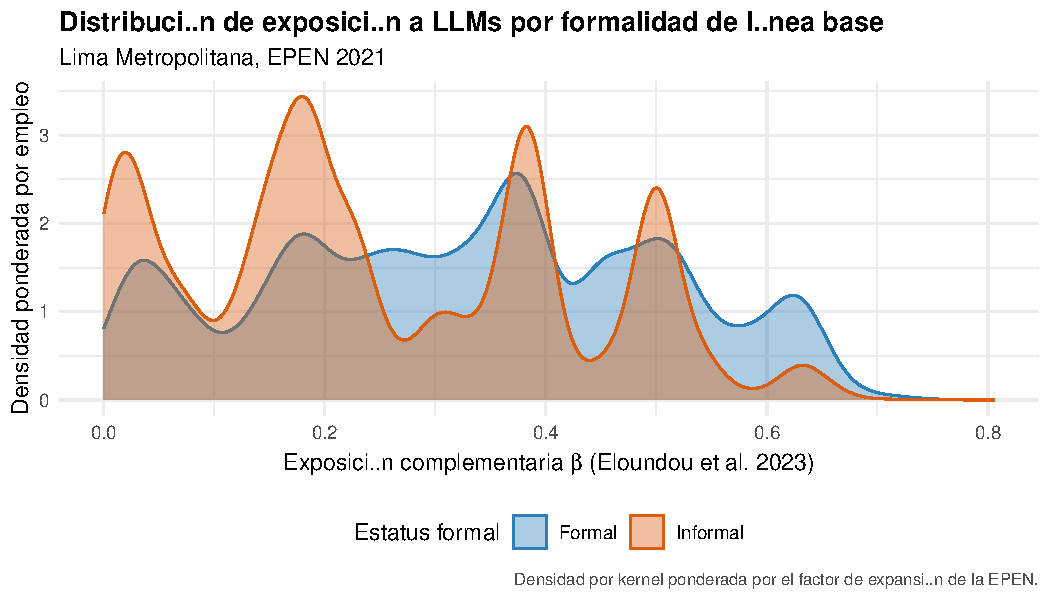
\includegraphics[width=0.85\textwidth]{figures/peru/fig_beta_distribution.pdf}
\caption{\textit{Densidad de la exposici\'{o}n complementaria $\beta$ por estatus de formalidad, Lima Metropolitana 2021.} La curva con relleno gris oscuro corresponde a trabajadores formales (\texttt{seguro1} $\in \{1, 3\}$) y la curva punteada con relleno gris claro a trabajadores informales. Las densidades est\'{a}n ponderadas por el factor de expansi\'{o}n trimestral de la EPEN.}
\label{fig:peru_beta_dist}
\end{figure}

Las dos colas de la distribuci\'{o}n est\'{a}n descritas en el \cref{app:peru_extremes}. La cola de alta exposici\'{o}n agrupa ocupaciones cognitivas profesionales (relaciones p\'{u}blicas, traductores, programadores de aplicaciones, escritores, matem\'{a}ticos, oficiales de cr\'{e}dito), todas concentradas en oficios cognitivos no rutinarios donde la sustituci\'{o}n parcial mediante software construido sobre LLM es plausible. La cola de baja exposici\'{o}n agrupa ocupaciones manuales y operativas (limpiadores de veh\'{i}culos, obreros de construcci\'{o}n, pintores, ayudantes de cocina), donde el contenido de tarea es f\'{i}sico y la complementariedad con LLM es estructuralmente baja.

La \cref{tab:peru_beta_formal} cruza los cuartiles de exposici\'{o}n con la share de formalidad para 2021 y entrega el hallazgo descriptivo m\'{a}s relevante para la estrategia de identificaci\'{o}n del art\'{i}culo: la formalidad se duplica entre el cuartil m\'{a}s expuesto y el menos expuesto. Las ocupaciones de alta exposici\'{o}n son sistem\'{a}ticamente m\'{a}s formales en la l\'{i}nea base.

\begin{table}[H]
\centering
\small
\begin{threeparttable}
\caption{Formalidad por cuartil de exposici\'{o}n $\beta$, Lima Metropolitana 2021}
\label{tab:peru_beta_formal}
\begin{tabular}{l c c c}
\toprule
Cuartil de $\beta$ & $\beta$ mediana & \% formal & Share del empleo (\%) \\
\midrule
Q1 (m\'{a}s baja)  & 0.034 & 25.8 & 25.1 \\
Q2                 & 0.188 & 30.0 & 25.4 \\
Q3                 & 0.375 & 41.0 & 25.6 \\
Q4 (m\'{a}s alta)  & 0.500 & 50.6 & 23.9 \\
\bottomrule
\end{tabular}
\begin{tablenotes}[flushleft]
\footnotesize
\item \emph{Notas:} Cuartiles de $\beta$ ponderados por empleo expandido en la EPEN 2021. La columna ``\% formal'' reporta la share de trabajadores con \texttt{seguro1} $\in \{1, 3\}$ dentro de cada cuartil.
\end{tablenotes}
\end{threeparttable}
\end{table}

\paragraph{Primeras conclusiones descriptivas.} Del cuadro descriptivo emergen tres patrones que orientan la estrategia de identificaci\'{o}n.

La exposici\'{o}n a LLMs en Lima Metropolitana resulta heterog\'{e}nea pero no extrema. La mediana ponderada por empleo es 0.255. La cola superior llega a 0.806 en relaciones p\'{u}blicas. La cola inferior concentra a un cuarto de los trabajadores en posiciones con $\beta = 0$. Esa distribuci\'{o}n no se concentra en un valor central. Ofrece, por lo mismo, variaci\'{o}n suficiente para estimar la dosis-respuesta a lo largo de la l\'{i}nea continua de tratamiento.

Un segundo patr\'{o}n, m\'{a}s relevante para la identificaci\'{o}n, es que los segmentos formal e informal de l\'{i}nea base ocupan posiciones distintas en la distribuci\'{o}n de exposici\'{o}n. La probabilidad de formalidad en una ocupaci\'{o}n del cuartil m\'{a}s expuesto (50.6 por ciento) duplica la del cuartil menos expuesto (25.8 por ciento). Esta correlaci\'{o}n est\'{a} predeterminada respecto al lanzamiento de ChatGPT, y por lo tanto refleja una caracter\'{i}stica estructural del mercado laboral peruano y no una respuesta al shock. Esa misma correlaci\'{o}n explica por qu\'{e} la heterogeneidad por formalidad es probablemente la dimensi\'{o}n con mayor magnitud emp\'{i}rica: la adopci\'{o}n de software complementario con LLM se concentra en firmas formales con capacidad de inversi\'{o}n y soporte tecnol\'{o}gico. Los efectos fijos de ocupaci\'{o}n absorben la correlaci\'{o}n de l\'{i}nea base y dejan la variaci\'{o}n intra-ocupaci\'{o}n como fuente del par\'{a}metro.

Un tercer hallazgo es que la propia composici\'{o}n ocupacional se est\'{a} desplazando lentamente hacia ocupaciones m\'{a}s expuestas durante el per\'{i}odo muestral. El $\beta$ medio ponderado por empleo sube de 0.280 en 2021 a 0.290 en 2025. El cambio es modesto. Aun as\'{i}, sugiere reasignaci\'{o}n a favor de ocupaciones expuestas, un margen extensivo cuya causalidad no es identificable directamente con esta especificaci\'{o}n pero que motiva el an\'{a}lisis de empleo expandido por celda en la \cref{sec:results}.

\paragraph{Construcci\'{o}n de celdas para el DiD.} Los microdatos armonizados se colapsan a la celda (CIUO-08 4d, trimestre) ponderando por empleo expandido. Se aplican dos filtros: las celdas con menos de 10 observaciones muestrales se descartan, y las ocupaciones que carecen completamente de observaciones en el per\'{i}odo pre o en el per\'{i}odo post se excluyen del an\'{a}lisis principal por requerir el estimador de \citet{CallawayCGBS2024_continuous} la presencia de la unidad en ambos per\'{i}odos. Tras aplicar estos filtros, el panel resultante para Per\'{u} contiene 138 ocupaciones CIUO-08 a cuatro d\'{i}gitos sobre 20 trimestres, para un total de 2{,}139 celdas (ocupaci\'{o}n, trimestre).

\section{Results}
\label{sec:results}

% Results section — to be written in Execution phase after primary DiD estimation.

\section{Robustness}
\label{sec:robustness}

% Robustness section — to be written in Execution phase.

\section{Conclusi\'{o}n}
\label{sec:conclusion}

Esta versi\'{o}n del art\'{i}culo presenta resultados preliminares para un solo pa\'{i}s. Se reportan las estimaciones causales para Per\'{u} (Lima Metropolitana, EPEN trimestral 2021T1--2025T4), construidas sobre el panel armonizado a CIUO-08 a cuatro d\'{i}gitos descrito en la \cref{sec:data}. La aplicaci\'{o}n del mismo dise\~{n}o a Costa Rica, Colombia, Ecuador, M\'{e}xico y Uruguay queda pendiente, y con ello tambi\'{e}n queda pendiente la comparaci\'{o}n entre pa\'{i}ses que constituye la contribuci\'{o}n emp\'{i}rica central del art\'{i}culo. Las afirmaciones a continuaci\'{o}n deben leerse como caracterizaci\'{o}n de Lima Metropolitana, no como evidencia regional para Am\'{e}rica Latina.

Tres conclusiones emergen de la evidencia peruana. Primero, la lectura agregada del shock de los LLMs en Lima Metropolitana es enga\~{n}osamente nula: la especificaci\'{o}n continua TWFE arroja coeficientes peque\~{n}os y estad\'{i}sticamente indistinguibles de cero al 95 por ciento sobre los tres resultados primarios, lo que en aislamiento sugerir\'{i}a una replicaci\'{o}n del nulo de \citet{HumlumVestergaard2025_llm}. La especificaci\'{o}n binaria de \citet{CallawayS2021_did} sobre la submuestra balanceada matiza esa lectura entregando un efecto positivo sobre el empleo ($+14.4$ por ciento, $p < 0.01$) y un efecto negativo sobre las horas semanales ($-0.80$, $p < 0.05$). La heterogeneidad por estimador es informativa por s\'{i} misma sobre las limitaciones de TWFE en presencia de respuestas heterog\'{e}neas a la dosis.

Segundo, la heterogeneidad por formalidad de l\'{i}nea base es la fuente principal del cuadro emp\'{i}rico. Los canales formal e informal se mueven en direcciones opuestas y estad\'{i}sticamente significativas en empleo ($\hat\tau_F = +0.567$ vs.\ $\hat\tau_I = -0.222$, test de igualdad $p = 0.005$) y en salario por hora ($\hat\tau_F = -0.128$ vs.\ $\hat\tau_I = +0.265$, test $p < 0.001$). Los nulos agregados emergen como resultado mec\'{a}nico de cancelaci\'{o}n entre canales con signos opuestos, no como evidencia de ausencia de efecto. La preregistraci\'{o}n de la formalidad como dimensi\'{o}n central de heterogeneidad queda emp\'{i}ricamente justificada.

Tercero, la lectura cualitativa peruana es consistente con una versi\'{o}n refinada de la \emph{Narrativa D} preregistrada. Las firmas formales que adoptan herramientas con LLM expanden el empleo en ocupaciones expuestas (margen extensivo positivo) y reducen las horas semanales por trabajador (ajuste intensivo). El sector informal experimenta contracci\'{o}n d\'{e}bil del empleo combinada con selecci\'{o}n positiva en salarios entre los trabajadores que permanecen en ocupaciones expuestas. Este cuadro contradice la lectura de complementariedad uniforme del sector formal de la OCDE y entrega un mecanismo distinto: complementariedad sesgada por habilidad, modulada por la segmentaci\'{o}n estructural del mercado laboral.

\paragraph{Limitaciones y trabajo en curso.} Cinco limitaciones del an\'{a}lisis actual orientan la versi\'{o}n siguiente del art\'{i}culo. Primero, el alcance geogr\'{a}fico de la EPEN restringe la representatividad a Lima Metropolitana, no al Per\'{u}. Segundo, la definici\'{o}n de formalidad basada en \texttt{seguro1} es una aproximaci\'{o}n por afiliaci\'{o}n a ESSALUD; la ENAHO anual permite una validaci\'{o}n con la definici\'{o}n est\'{a}ndar OIT basada en pensiones. Tercero, la armonizaci\'{o}n del clasificador ocupacional descansa en pesos posteriores emp\'{i}ricos cuya sensibilidad a esquemas alternativos ser\'{a} contrastada en la escalera de robustez de la \cref{tab:peru_classifier_ladder}. Cuarto, las medidas alternativas de exposici\'{o}n ($\alpha$, $\zeta$, Webb, Felten) y el donut DiD que excluye los trimestres adyacentes al cambio de clasificador permanecen como verificaciones pendientes en la secci\'{o}n de robustez. Quinto, y de orden mayor, los pa\'{i}ses restantes del art\'{i}culo (Costa Rica, Colombia, Ecuador, M\'{e}xico y Uruguay) requieren la replicaci\'{o}n del pipeline para entregar las seis estimaciones $\{\hat\tau^c\}_{c=1}^6$ que constituyen el resultado principal preregistrado.

La versi\'{o}n final del art\'{i}culo contrastar\'{a} los seis pa\'{i}ses lado a lado e identificar\'{a} cu\'{a}l de las cuatro narrativas preregistradas se sostiene en cada pa\'{i}s. Los resultados peruanos sugieren que el agregado regional puede esconder heterogeneidades de signo entre canales formal e informal que merecen estimaci\'{o}n separada en cada pa\'{i}s, y que la evidencia causal sobre el efecto laboral de los LLMs en Am\'{e}rica Latina probablemente difiera de las primeras estimaciones causales de econom\'{i}as de la OCDE no por replicaci\'{o}n del nulo, sino por la mediaci\'{o}n de instituciones de mercado laboral espec\'{i}ficas de la regi\'{o}n.


\clearpage
\small \printbibliography

\end{document}
